\documentclass[aspectratio=169]{beamer}
\usepackage{fontspec}
\usepackage{blindtext}

\setmainfont{Calibri}
\title{There Is No Largest Prime NumbePrime NumbePrime Number}
\subtitle{A very very ververy very very very very very very very long subtitle}
\date{\today}
\author[Euclid]{Euclid of Alexandria \texttt{euclid@alexandria.edu}}

\usetheme[titlepage=4]{siegen}
\usecolortheme{nt}

\titlegraphic{
    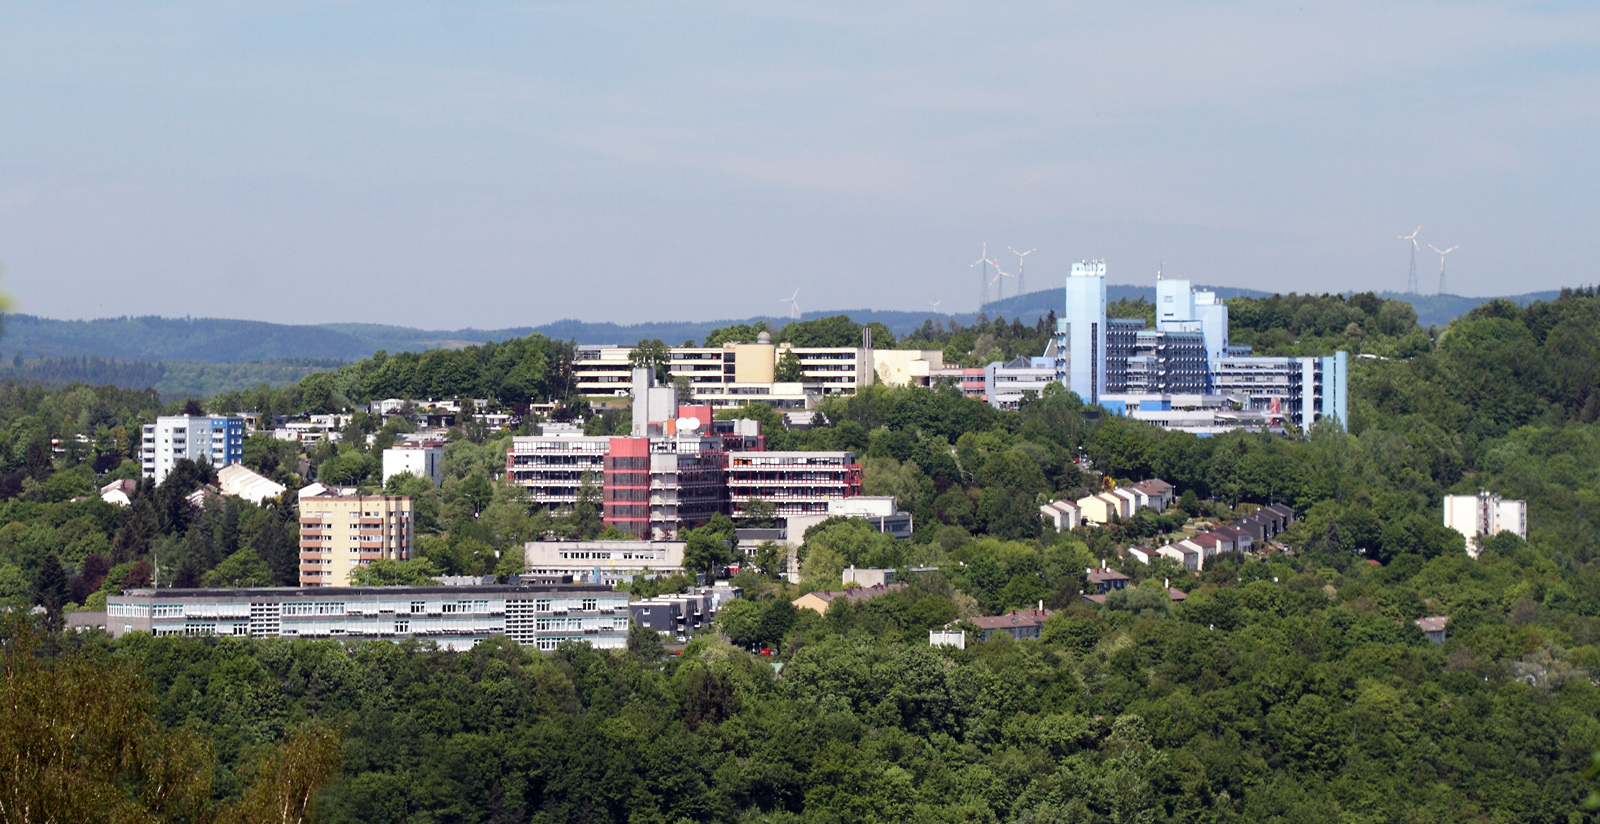
\includegraphics[height=\paperheight,width=\paperwidth]{img/progress.jpg}
}

\begin{document}
	
%	\section{LLL}
%	\subsection{kakak}

\begin{frame}
\titlepage
\end{frame}

%\section{test}

\begin{frame}{testasd asdj oasjdkdj asdj aksdjadsj apsd jaods testasd asdj oasjdkdj oads testasd asdj oasjdkdj asdj aksdjadsj apsd jaods testaad j}
	
	\framesubtitle{The proof uses \textit{reductio ad absurdum}.} 
	\blindtext
\end{frame}

\part{Hier steht der Kapitelname}

\end{document}

